\documentclass[12pt,UTF8]{ctexbook}
\usepackage{ctex}
\usepackage{caption}
\usepackage{graphicx}
\usepackage{float}
\usepackage{wrapfig}
\usepackage{array}
\usepackage[table, dvipsnames, svgnames, x11names]{xcolor}
\usepackage{colortbl}% 
\usepackage{tabularx}
\usepackage{amsmath}
\usepackage{amssymb}
\usepackage{xfrac}
\usepackage{eucal}
\usepackage{titlesec}
\usepackage{amsthm}
\usepackage{tikz-cd}
\usepackage{enumitem}
\usepackage{verbatim}
\usepackage{fontspec,xunicode,xltxtra}
\usepackage{xeCJK} 
\usepackage[b]{esvect}

\definecolor{gl}{RGB}{246, 252, 240}
\definecolor{gd}{RGB}{236, 244, 230}
\definecolor{bg}{RGB}{242, 244, 228}


\setCJKmainfont[BoldFont=STZhongsong]{STSong}
\setCJKmonofont{simkai.ttf} % for \texttt
\setCJKsansfont{simfang.ttf} % for \textsf
\setlength\parskip{8pt}
\setlength{\fboxsep}{12pt}
\renewcommand\thesection{\arabic{chapter}.\arabic{section}}
\newtheorem{df}{定义}[section] 
\newtheorem{pp}{命题}[section]
\newtheorem{tm}{定理}[section]
\newtheorem{ex}{例子}[section]
\newtheorem{sk}{思考}[section]
\newtheorem{po}{公理}
\newtheorem*{so}{解答}
\newenvironment{proof2}{\paragraph{\textbf{证明:}}}{\hfill$\square$}
\newtheorem{xt}{习题}[section]
\newtheorem{cor}{推论}[pp]
\renewcommand{\proofname}{\indent\bf 证明}
\renewcommand{\qedsymbol}{\hfill$\square$}
% 列举环境的行间距
\setenumerate[1]{itemsep=0pt,partopsep=0pt,parsep=0pt,topsep=0pt}
\setitemize[1]{itemsep=0pt,partopsep=0pt,parsep=0pt,topsep=0pt}
\setdescription{itemsep=0pt,partopsep=0pt,parsep=0pt,topsep=0pt}
\setlength{\intextsep}{2pt}%
\setlength{\columnsep}{2pt}%
% 新函数
\renewcommand\parallel{\mathrel{/\mskip-4mu/}}
% 章节字体大小
\titleformat{\section}{\zihao{-2}\bfseries}{ \thesection }{16pt}{}
% 封面
\title{\zihao{0} \bfseries 第六册}
\author{\zihao{2} \texttt{大青花鱼}}
% \date{\bfseries\today}
\date{}
% 正文
\begin{document}
\maketitle
\tableofcontents
\newpage

\chapter{向量}
第五册中,我们学习了用三角函数解三角形。三角函数是定量研究平面形的利器。
不过,三角函数本身并不是简单的函数。我们目前只能通过查表的方式得到函数值。
这让我们思考,能不能打造一种更方便定量研究的体系呢?

回顾我们对平面形的研究,我们从几条公理出发,得出点、直线、三角形、圆等形状之间的定性关系。
公理体系的缺陷在于没有与数紧密结合。比如,“两点之间直线最短”,除了定性的“最短”,没有提供别的信息。
我们需要一种根本上和数量结合的体系,来理解各种平面形状。

此外,公理体系中并没有强调运动的概念。我们说点运动形成了线,旋转形成角度和圆,
但并没有相关的工具来描述具体的运动。我们需要一种根本上和运动结合的体系,来理解形状之间的关系。

\section{点、向量和直线}
学习有理数的时候,我们使用数轴上的点表示。每个点代表一个实数。两点重合,
当且仅当它们代表同一个数。这种表示方法把数和直线上的点牢牢绑在一起。
我们可以用数的关系表示直线上点的关系。数轴使我们可以定量理解直线。

至于平面中的点,我们用相互垂直的数轴定义了点的坐标。每个点代表一个有序数对。两个数按顺序排列,对应平面中一点。

能不能像数轴一样,用一个量代表平面中一点呢?数轴之所以能用一个数代表一个点,
是因为直线只有两个方向,使用正负号就可以代表方向。平面中不止两个方向,我们无法用正负来表示方向了。
为此,我们引入一个新的量来代表平面中的点:\textbf{向量}。

自然数、有理数、实数都有自己的运算法则。向量作为代表点的量,需要满足怎样的运算法则呢?
我们从运动出发,给出以下的法则:
\begin{enumerate}
    \item 向量的加法就是平移:两个向量相加得到另一个向量。向量的加法满足结合律和交换律。
    \item 零向量表示静止不变:存在这样一个向量,任何向量与它相加,仍然是自己。
    这个向量叫做\textsl{零向量}。零向量不定义方向,也可以说它与任何向量同向或反向。它对应的点称为\textbf{原点}。
    \item 从每个非零向量,引出一根数轴:任何实数乘以向量,得到方向相同或相反的向量。
    这个运算称为\textbf{数乘运算}。数乘运算对应图形的放缩。
    \item 放缩和四则运算相容:数轴上可以做数的运算。
    \item 平移和放缩相容:先平移再放缩,和先放缩再平移,结果一样。
\end{enumerate}
按照定义,\textbf{向量就是点},所以可以用大写字母来表记。比如零向量就是原点,记为$O$。
此外,\textbf{向量就是平移}。点$A$就是把$O$对应到$A$的平移,也是$O$平移的结果,记为$\vv  {OA}$。
反过来,$\vv  {BA}$就是把$B$对应到$A$的平移。

让我们用数学语言把这些法则更具体地写出来。我们把平面看作集合,记为$\mathbb{V}$,其中的元素称为向量或点,
用粗体小写字母表示,以便和代表数的量区分:
\begin{enumerate}
    \item 加法结合律:$\forall \,\, \mathbf{a}, \mathbf{b}, \mathbf{c} \in \mathbb{V}$,$\mathbf{a}+ (\mathbf{b} + \mathbf{c}) = (\mathbf{a} + \mathbf{b}) + \mathbf{c}$。
    \item 加法交换律:$\forall \,\, \mathbf{a}, \mathbf{b} \in \mathbb{V}$,$\mathbf{a} + \mathbf{b} = \mathbf{b} + \mathbf{a}$。
    \item 存在零向量:$\forall \,\, \mathbf{a} \in \mathbb{V}$,$\mathbf{a} + \mathbf{0} = \mathbf{a}$。
    \item 放缩和四则运算相容:$\forall \,\, \mathbf{a} \in \mathbb{V}$,$1\cdot \mathbf{a} = \mathbf{a}$。$\forall s, t \in \mathbb{R}$,$(s + t)\cdot\mathbf{a} = (s\cdot\mathbf{a}) + (t\cdot\mathbf{a})$,$(s \cdot t)\cdot \mathbf{a} = s \cdot (t\cdot \mathbf{a})$。
    \item 放缩和平移相容:$\forall \,\, \mathbf{a}, \mathbf{b} \in \mathbb{V}$,$\forall \,\, t \in \mathbb{R}$,$t\cdot(\mathbf{a} + \mathbf{b}) = t\cdot\mathbf{a} + t\cdot\mathbf{b}$。
\end{enumerate}

从以上法则出发,我们可以定义直线:
\begin{df}
    过原点的直线是非零向量放缩得到的集合。不过原点的直线是过原点的直线按一点平移得到的集合。
\end{df}
给定非零向量$A = \mathbf{a}$,$ \{t\mathbf{a} \, | \, t\in\mathbb{R}\}$是一条过原点$O$和$A$的直线$OA$。
给定向量$B = \mathbf{b}$,$ \{t\mathbf{a}+\mathbf{b} \, | \, t\in\mathbb{R}\}$是一条过$B$的直线;
而$ \{t\mathbf{a}+(1 - t)\mathbf{b} \, | \, t\in\mathbb{R}\}$就是直线$AB$。

给定非零向量$\mathbf{a}$,如果向量$\mathbf{b}$可以通过$\mathbf{a}$放缩得到,
或者说$\mathbf{b}\in \{t\mathbf{a} \, | \, t\in\mathbb{R}\}$,就称两者\textbf{共线}。

类比可以定义线段和射线:给定非零向量$A = \mathbf{a}$和向量$B =\mathbf{b}$,
$ \{t\mathbf{a}+(1 - t)\mathbf{b} \, | \, t\in [0, 1]\}$是端点为$\mathbf{a}, \mathbf{b}$的线段$AB$,
$ \{t\mathbf{a}+(1 - t)\mathbf{b} \, | \, t \geqslant 0 \}$是以$B$为端点,经过$A$的射线。

这样定义的线段和射线,也具备了数轴的性质。比如,在线段$\{t\mathbf{a}+(1 - t)\mathbf{b} \, | \, t\in [0, 1]\}$
中,$t$的不同值就对应了不同的点:$t = 0$对应点$\mathbf{b}$,$t=1$对应点$\mathbf{a}$。对一般的$t\in (0, 1)$,
$t\mathbf{a}+(1 - t)\mathbf{b}$对应的点$P(t)$满足:$|AP(t)| = (1 - t)|AB|$,$|P(t)B| = t|AB|$。也就是说,
$P(t)$是线段$AB$上使得$ \frac{|AP(t)|}{|P(t)B|} = \frac{1 - t}{t}$的点。
$\vv{AP(t)}, \vv{P(t)B}$都和$\vv{AB}$共线。

反过来,设$ \frac{|AP(t)|}{|P(t)B|}$等于定值$k > 0$,对应的点$P(t)$是什么点呢?
这个问题实际上是求方程:
$$ \frac{1 - t}{t} = k$$
的解。容易解出这个方程的唯一解:$t = \frac{1}{k+1}$。因此我们得到结论:
\begin{tm}{\textbf{定比分点定理} }\label{tm:0-0-10}
    线段$AB$上到两端距离之比$\frac{|AP|}{|PB|}$为定值$k$的点$P$恰有一个,称为它的$k$\textbf{分点}。
\end{tm}
正数$k$越小,$k$分点距离$A$越近,$k$越大,$k$分点离$A$越远;$k=1$时,我们就得到线段的中点。

以上我们讨论了$k>0$的情况,显然,$k=0$对应$P = A$。对于负数$k$,有没有对应的点呢?
我们用平移的思想考虑这个问题,从$A$到$P(t)$经历的平移是$\vv{AP(t)} = (1 - t)\vv{AB}$,
从$P(t)$到$B$经历的平移是$\vv{P(t)B} = t\vv{AB}$。它们的系数之比就是$ \frac{1 - t}{t}$。
于是,我们可以对一般的$k$定义定比分点:如果$k$能使得方程
$$ \frac{1 - t}{t} = k$$
有唯一解,那么我们就把对应的点$P(t)$称为$AB$的$k$分点。

如果$k<-1$,那么$k$分点对应的$t = \frac{1}{k+1} < 0$,也就是说,$P(t)$在线段$BA$沿$B$的延长线上。
如果$-1<k<0$,那么$k$分点对应的$t = \frac{1}{k+1} > 1$,也就是说,$P(t)$在线段$BA$沿$A$的延长线上。
如果$k=-1$,以上方程无解,这说明$-1$分点不存在。

共线的向量,通过数轴,可以方便地讨论相互的位置关系。不共线的向量之间,
如何讨论位置关系呢?为此,我们要引入\textbf{平面的根本性质}:
\begin{enumerate}
    \item 给定任何非零向量$A$,平面中总有另一个向量$B$,不在直线$OA$上。我们说两者\textbf{不共线}。
    \item 从不共线的向量$A, B$出发,经过放缩、平移,可以得到平面中任何向量。具体来说,
    任何向量都可以表示成$sA + tB$的形式,集合$\{sA + tB | s, t, \in\mathbb{R}\}$就是整个平面。
    这样的$A, B$称为平面的一组\textbf{基}或\textbf{基底}。
\end{enumerate}

举例来说,在直角坐标系中,我们选择了原点重合、互相垂直的两条数轴,以每条数轴上数$1$对应的点(记为$\mathbf{e}_x, \mathbf{e}_y$)出发,通过放缩和平移,
就得到平面所有的点。平面中任一点可以写成$x\mathbf{e}_x + y\mathbf{e}_y$,其中$x,y$就是点的坐标。
直角坐标系其实是一种用向量描述平面的方法。$\mathbf{e}_x, \mathbf{e}_y$就是一组基。

\begin{sk}\label{sk:0-0-10}
    \mbox{}\\
    1. 设平面上有两点$A,B$,以$OA, OB$为邻边作平行四边形$AOBC$。向量$\vv{OA}$和$\vv{BC}$是什么关系?\\
    2. 设平面上有两点$A,B$,三角形$OAB$中,连接边$OA, OB$的中点$M,N$。向量$\vv{AB}$和$\vv{MN}$是什么关系?
\end{sk}
\begin{xt}\label{xt:0-0-10}
    \mbox{} \\
    \indent 1. 证明:零向量只有一个,任何向量乘$0$得到零向量。\\
    \indent 2. 证明:零向量乘任何数得到零向量。\\
    \indent 3. 证明:任何向量$\mathbf{a}$都有唯一的反向量$\mathbf{b}$,满足$\mathbf{a} + \mathbf{b} = \mathbf{0}$。\\
    \indent 4. 设$\mathbf{a}, \mathbf{b}$不共线,如果$s\mathbf{a} + t\mathbf{b} = \mathbf{0}$,证明:$s = t = 0$。\\
    直角坐标系$xOy$中,设$\mathbf{a} = 4\mathbf{e}_x + \mathbf{e}_y$,$\mathbf{b} = \mathbf{e}_x - 2\mathbf{e}_y$
    ,$\mathbf{b} = -\mathbf{e}_x + 2\mathbf{e}_y$。\\
    \indent 5. 在坐标轴上标出$\mathbf{a}$,$\mathbf{b}$和$\mathbf{c}$。\\
    \indent 6. 用$\mathbf{a}$和$\mathbf{b}$表示$\mathbf{e}_x$、$\mathbf{e}_y$和点$(3,0)$。\\
    \indent 7. 用$\mathbf{a}$和$\mathbf{b}$表示它们的中点、$3$分点、$-0.5$分点、$-3$分点。
    写出这些点的坐标和直线的方程。\\
    \indent 8. 用$\mathbf{a}, \mathbf{b}, \mathbf{c}$表示顶点为$\mathbf{a}, \mathbf{b}, \mathbf{c}$的三角形三边和重心。
\end{xt}

\section{角度与长度}
根据平面的根本性质,任何向量都可以用两个不共线向量表示。如何讨论它们的位置关系呢?
下面我们定义一种关系,把长度、距离和角度统一起来。

给定平面基底$\mathbf{e}_1, \mathbf{e}_2$,我们给出这样一个二元映射$f$:
$$ \forall \,\, \mathbf{a} = x_A\mathbf{e}_1 + y_A\mathbf{e}_2, \,\, \mathbf{b} = x_B\mathbf{e}_1 + y_B\mathbf{e}_2, \,\, \in \mathbb{R}, \quad f(\mathbf{a}, \mathbf{b}) = x_Ax_B + y_Ay_B.$$
$f$把两个向量对应到一个实数。它满足以下五个性质:
\begin{enumerate}
    \item 向量的顺序不影响关系大小:
    \begin{align}
         & f(x_A\mathbf{e}_1 + y_A\mathbf{e}_2, x_B\mathbf{e}_1 + y_B\mathbf{e}_2) \notag \\
        =\,\,& x_Ax_B + y_A y_B = x_Bx_A + y_By_A \notag \\
        =\,\,& f(x_B\mathbf{e}_1 + y_B\mathbf{e}_2, x_A\mathbf{e}_1 + y_A\mathbf{e}_2). \notag
    \end{align}
    \item 零向量和任意向量关系为$0$:
    $$f(x_A\mathbf{e}_1 + y_A\mathbf{e}_2, \mathbf{0}) = f(x_A\mathbf{e}_1 + y_A\mathbf{e}_2, 0\mathbf{e}_1 + 0\mathbf{e}_2) = x_A\cdot 0 + y_A\cdot 0 = 0.$$
    \item 非零向量与自身的关系总是正的:$x_A, y_A$不全为零时,
    $$f(x_A\mathbf{e}_1 + y_A\mathbf{e}_2, x_A\mathbf{e}_1 + y_A\mathbf{e}_2) = x_A^2 + y_A^2  > 0.$$
    \item 和向量的放缩相容:
    \begin{align}
        & f(x_A\mathbf{e}_1 + y_A\mathbf{e}_2, t(x_B\mathbf{e}_1 + y_B\mathbf{e}_2)) \notag \\
        =\,\,& x_Atx_B + y_A ty_B = t(x_Ax_B + y_Ay_B) \notag \\
        =\,\,& tf(x_A\mathbf{e}_1 + y_A\mathbf{e}_2, x_B\mathbf{e}_1 + y_B\mathbf{e}_2). \notag 
    \end{align}
    \item 和向量的平移相容:
    \begin{align}
         & f(x_A\mathbf{e}_1 + y_A\mathbf{e}_2, (x_B\mathbf{e}_1 + y_B\mathbf{e}_2) + (x_C\mathbf{e}_1 + y_C\mathbf{e}_2)) \notag \\
         =\,\,& x_A(x_B + x_C) + y_A (y_B + y_C) = (x_Ax_B + y_Ay_B) + (x_Ax_C + y_Ay_C) \notag \\
         =\,\,& f(x_A\mathbf{e}_1 + y_A\mathbf{e}_2, x_B\mathbf{e}_1 + y_B\mathbf{e}_2) + f(x_A\mathbf{e}_1 + y_A\mathbf{e}_2, x_C\mathbf{e}_1 + y_C\mathbf{e}_2). \notag
    \end{align}     
\end{enumerate}
满足以上五个条件的映射$f$称为平面向量的\textbf{内积}。从第四个性质可知,向量与自身的内积总是正数。
我们把这个数的平方根叫做向量的长度,记为:
$$ \forall \,\, \mathbf{a} \in \mathbb{V}, \quad \| \mathbf{a}\| = \sqrt{f(\mathbf{a}, \mathbf{a})}. $$
两个向量之差的长度,称为向量之间的距离。
$$ \forall \,\, \mathbf{a}, \mathbf{b} \in \mathbb{V}, \quad \| \mathbf{a} - \mathbf{b}\| = \sqrt{f(\mathbf{a} - \mathbf{b}, \mathbf{a} - \mathbf{b})}. $$
如果基底$\mathbf{e}_1, \mathbf{e}_2$是直角坐标系的基,那么
\begin{align}
    \forall \,\, \mathbf{a} = x_A\mathbf{e}_x &+ y_A\mathbf{e}_y , \notag \\
    \| \mathbf{a}\| &= \sqrt{x_A^2 + y_A^2}, \notag \\
    \forall \,\, \mathbf{a} = x_A\mathbf{e}_x &+ y_A\mathbf{e}_y,\,\,\, \mathbf{b} = x_B\mathbf{e}_x + y_B\mathbf{e}_y , \notag \\
    \| \mathbf{a} - \mathbf{b}\| &= \sqrt{(x_A - x_B)^2 + (y_A - y_B)^2}. \notag
\end{align}
给定向量$A = \mathbf{a}$、$B =\mathbf{b}$,$\| \mathbf{a} \|$就是$|OA|$,
$\|\mathbf{a} - \mathbf{b}\|$就是$|AB|$。
也就是说,我们这样定义的映射$f$,分别与直观经验中长度和距离的概念相符合。

那么,$f$本身有什么含义呢?我们来计算$ \frac{|OA|^2 + |OB|^2 - |AB|^2}{2}.$
\begin{align}
    \frac{|OA|^2 + |OB|^2 - |AB|^2}{2} &= \frac{x_A^2 + y_A^2 + x_B^2 + y_B^2 - (x_A - x_B)^2 - (y_A - y_B)^2}{2} \notag \\
    &= x_Ax_B + y_Ay_B = f(\mathbf{a}, \mathbf{b}). \notag 
\end{align}
另一方面,余弦定理告诉我们,$ \frac{|OA|^2 + |OB|^2 - |AB|^2}{2} = |OA||OB|\cos \angle AOB$。
也就是说,$f(\mathbf{a}, \mathbf{b}) = \|\mathbf{a}\| \|\mathbf{b}\| \cos \angle AOB$。% \langle \mathbf{a}, \mathbf{b}\rangle 
内积$f$的本质是向量夹角的余弦与向量长度的乘积。通过内积,我们把角度和长度统一起来了。

向量夹角的余弦值总在$-1$和$1$之间,所以向量的内积的绝对值不大于向量长度的乘积:
$$ |x_Ax_B + y_Ay_B| \leqslant \sqrt{x_A^2 + y_A^2} \sqrt{x_B^2 + y_B^2}.$$
可以验证这个关系对任意$x_A, y_A, x_B, y_B$成立。从这个关系出发,可以得到:
$$ |AB| = \sqrt{(x_A - x_B)^2 + (y_A - y_B)^2} \leqslant \sqrt{x_A^2 + y_A^2} + \sqrt{x_B^2 + y_B^2} = |OA| + |OB|.$$
这符合直观经验中“三角形两边之和大于第三边”或“两点之间线段距离最短”的性质。

内积为$0$,就表示向量夹角的余弦为$0$,即两个向量垂直。
比如令$\mathbf{a} = 2\mathbf{e}_x - \mathbf{e}_y$,$\mathbf{b} = \mathbf{e}_x + 2\mathbf{e}_y$,
那么$f(\mathbf{a}, \mathbf{b}) = 2\cdot 1 - 1\cdot 2 = 0$。在平面上画出对应的点$A,B$,
可以验证$\angle AOB = 90^\circ$。

内积映射并不是唯一的,我们看另一个映射$f_2$:
$$ \forall \,\, x_A, y_A, x_B, y_B \in \mathbb{R}, \quad f(x_A\mathbf{e}_1 + y_A\mathbf{e}_2, x_B\mathbf{e}_1 + y_B\mathbf{e}_2) = 2x_Ax_B + y_A y_B.$$
可以验证,$f_2$也满足$f$满足的五个性质。从$f_2$出发,我们也可以定义距离和长度:
$$ \forall \,\, \mathbf{a} = x_A\mathbf{e}_x + y_A\mathbf{e}_y, \quad \| \mathbf{a} \|_2 = f_2(\mathbf{a}, \mathbf{a}) = 2x_A^2 + y_A^2. $$
这样定义的距离和长度和我们直观经验中有些不一样,不过,我们可以验证,这样定义的距离也满足“两点之间线段最短”的性质。
$$ |2x_Ax_B + y_Ay_B| \leqslant \sqrt{2x_A^2 + y_A^2} \sqrt{2x_A^2 + y_A^2}.$$
因此,$f_2$也是内积。

我们把符合直观经验的内积$f$称为\textbf{经典内积},一般称内积都默认指经典内积;
把对应的长度称为向量的\textbf{模}。
我们把$\mathbf{a}, \mathbf{b}$的(经典)内积记为$(\mathbf{a}\, | \, \mathbf{b})$,
不至于混淆时,也常称为\textbf{点积},记为$\mathbf{a} \cdot \mathbf{b}$;
把它们的模记为$|\mathbf{a}|$、$|\mathbf{b}|$。

既然有余弦,自然有正弦。记$\alpha = \angle AOB$,
则$(\mathbf{a}\, | \, \mathbf{b}) = |\mathbf{a}||\mathbf{b}| \cos \alpha$,
于是,
$$ |\mathbf{a}|^2|\mathbf{b}|^2 \sin^2 \alpha = |\mathbf{a}|^2|\mathbf{b}|^2 - (\mathbf{a}\, | \, \mathbf{b})^2 $$
记$\mathbf{a} = x_A\mathbf{e}_x + y_A\mathbf{e}_y$,$\mathbf{b} = x_B\mathbf{e}_x + y_B\mathbf{e}_y$,
则
\begin{align}
    (x_A^2 + y_A^2)(x_B^2 + y_B^2) \sin^2 \alpha &= (x_A^2 + y_A^2)(x_B^2 + y_B^2) - (x_Ax_B + y_Ay_B)^2 \notag \\
    &= (x_Ay_B - x_By_A)^2 \notag \\
    |\sin \alpha| &= \frac{|x_Ay_B - x_By_A|}{\sqrt{x_A^2 + y_A^2} \sqrt{x_B^2 + y_B^2}} \notag
\end{align}
我们得出了夹角$\angle AOB$正弦的绝对值。

观察向量夹角的正弦和余弦,我们注意到,它们的表达式与和差角公式有相似之处。
$x_Ax_B + y_Ay_B$与差角余弦公式形式相似,$x_Ay_B - x_By_A$与差角正弦公式形式相似。

让我们在直角坐标系中找几个例子,看看直观结果。设有点$A(1,\,\,0)$、$B(\frac{1}{2},\frac{\sqrt{3}}{2})$。
不难得出$\angle AOB = 60^\circ$。我们用以上公式计算$\angle AOB$的正弦和余弦:
$$ \frac{x_Ay_B - x_By_A}{\sqrt{x_A^2 + y_A^2}\sqrt{x_B^2 + y_B^2}} = \frac{\sqrt{3}}{2}, \quad \frac{x_Ax_B + y_Ay_B}{\sqrt{x_A^2 + y_A^2} \sqrt{x_B^2 + y_B^2}} = \frac{1}{2}. $$
把$P$的坐标换成$(0,\,\,1)$、$(-\frac{\sqrt{2}}{2}, \frac{\sqrt{2}}{2})$、$(\frac{\sqrt{3}}{2},-\frac{1}{2})$等,
我们发现,通过以上两个公式得到的值,就是$\angle AOB$的正弦、余弦值。
记$\angle AOB = \alpha$,那么:
$$ \sin \alpha = \frac{x_Ay_B - x_By_A}{\sqrt{x_A^2 + y_A^2}\sqrt{x_B^2 + y_B^2}}, \quad \cos \alpha = \frac{x_Ax_B + y_Ay_B}{\sqrt{x_A^2 + y_A^2} \sqrt{x_B^2 + y_B^2}}. $$

% 要注意的是,以上公式成立,是因为直角坐标系$xOy$的$x$轴和$y$轴沿逆时针顺序摆放,同时规定逆时针方向为角度的正方向。
% 如果直角坐标系的坐标轴摆放顺序和角度的正方向相反,以上的公式就要改为:
% $$ \sin \alpha = \frac{x_By_A - x_Ay_B}{\sqrt{x_A^2 + y_A^2}\sqrt{x_B^2 + y_B^2}}, \quad \cos \alpha = \frac{x_Ax_B + y_Ay_B}{\sqrt{x_A^2 + y_A^2} \sqrt{x_B^2 + y_B^2}}. $$

我们是通过面积定义正弦的。比如,邻边为$OA$和$OB$的平行四边形,面积是$|OA||OB|\sin \angle AOB$。
对照上面正弦的表达式,可以发现这个面积等于$x_Ay_B - x_By_A$。于是,我们把对应的映射
$$ (\mathbf{a}, \,\,\mathbf{b}) \mapsto x_Ay_B - x_By_A. $$
称为向量$A, B$的\textbf{面积},记为$\mathbf{a} \wedge \mathbf{b}$。

向量的面积和内积,分别对应正弦和余弦。两向量面积为零,当且仅当它们共线;两向量内积为零,当且仅当它们互相垂直。

\begin{xt}
    \mbox{} \\
    1. 直角坐标系中,已知两向量,计算它们的内积和面积,讨论它们的关系。\\
    \indent 1.1. $A(0,\,\, 2), \,\,\, B(1, \,\,1)$ \\
    \indent 1.2. $A(2,\,\, 1),\,\,\,  B(0.5, \,\,-1)$ \\
    \indent 1.3. $A(1.6,\,\, 0.2), \,\,\, B(-0.9,\,\, -3)$\\
    \indent 1.4. $A(1, \,\,-0.28), \,\,\, B(-0.45,\,\, -0.6)$\\
    2. 直角坐标系中,已知向量$B$的模为$2$,根据以下条件,求向量$A,B$的内积:\\
    \indent 2.1 $A = (-4, \,\,2), \,\,\, \angle AOB = 60^\circ$\\
    \indent 2.2 $A= (0,\,\, 5), \,\,\,\angle AOB = 135^\circ$\\
    \indent 2.3.$A = (3,\,\, -2.5), \,\,\,\angle AOB = 45^\circ$\\
    3. 直角坐标系中,已知点$P(2,\,\,1)$,求使得$P,Q$内积为$4$的点$Q$。\\
    4. 直角坐标系中,已知点$P(2,\,\,1)$,求使得$P,Q$面积为$4$的点$Q$。
\end{xt}

\begin{sk}
    如果直角坐标系$xOy$的$x$轴和$y$轴沿逆时针排布,而角度的正方向为顺时针方向,角$\alpha$的正弦和余弦是否还能写成
    $$ \sin \alpha = \frac{x_Ay_B - x_By_A}{\sqrt{x_A^2 + y_A^2}\sqrt{x_B^2 + y_B^2}}, \quad \cos \alpha = \frac{x_Ax_B + y_Ay_B}{\sqrt{x_A^2 + y_A^2} \sqrt{x_B^2 + y_B^2}}$$
    的形式?
\end{sk}

\section{直线的方程}

直角坐标系中,任意给定二元一次方程$ax + by + c = 0$($a$、$b$不全为$0$),
它的解集都对应平面中一条直线。我们把这个二元一次方程称为直线的\textbf{一般式}方程。
比如,$3x - 2y + 1 = 0$就是一条直线的一般式方程。不过,从这个式子,我们不容易看出相应的直线有什么性质。

下面我们用向量的语言,给出有不同直观性质的直线的方程。

\textbf{点向式}:已知直线过点$A(x_A,\,\, y_A) = \mathbf{a}$,方向为$\mathbf{b} = (x_B,\,\, y_B)$。
考虑直线上一点$P(x,\,\, y) = \mathbf{p}$,$\mathbf{p} - \mathbf{a}$和$\mathbf{b}$共线,所以面积为$0$。
于是$(x,\,\,y)$满足方程:
$$(x - x_A) y_B - (y - y_A) x_B = 0.$$
我们把这个二元一次方程称为直线的点向式方程。已知直线上一点和直线的方向,可以写出直线的点向式方程。
比如,过$(1,\,\,2)$,方向为$(-1,\,\,1)$的直线方程为:$1\cdot(x - 1) - (-1)\cdot(y - 2) = 0$,即$x + y = 3$。

\textbf{两点式}:已知直线过点$A(x_A,\,\, y_A) = \mathbf{a}$和点$B(x_B,\,\, y_B) = \mathbf{b}$。
考虑直线上一点$P(x,\,\, y) = \mathbf{p}$,则$\mathbf{p} - \mathbf{a}$和$\mathbf{b} - \mathbf{a}$共线。
于是$(x,\,\,y)$满足方程:
$$(x - x_A) (y_B - y_A) - (y - y_A) (x_B - x_A) = 0.$$
我们把以上方程称为直线的两点式方程。已知直线上不同的两点,可以写出直线的两点式方程。比如,
过$(1,\,\,2)$、$(-2,\,\,1)$的直线方程为:$(x - 1)(1 - 2) - (y - 2)(-2 - 1) = 0$,即$-x + 3y = 5$。

\textbf{点斜式}:已知直线过点$A(x_A,\,\, y_A) = \mathbf{a}$,斜率为$k$。
考虑直线上一点$P(x,\,\, y) = \mathbf{p}$。
直线斜率为$k$,说明直线是某个一次函数$x \mapsto kx + b$的图像。对比可知,直线方向和$(1,\,\,k)$共线。
我们用$(1,\,\,k)$作为直线方向,于是直线方程为:
$$y - y_A = k(x - x_A).$$
我们把这个方程称为直线的点斜式方程。已知直线上一点和直线的斜率,可以写出直线的点斜式方程。
比如,过$(1,\,\,2)$,斜率为$2$的直线方程为:$y - 2 = 2(x - 1)$,即$y - 2x = 0$。

\textbf{点法式}:已知直线过点$A(x_A,\,\, y_A) = \mathbf{a}$,并且和$\mathbf{b} = (x_B,\,\, y_B)$垂直。
考虑直线上一点$P(x,\,\, y) = \mathbf{p}$,$\mathbf{p} - \mathbf{a}$和$\mathbf{b}$垂直,所以内积为$0$。
于是$(x,\,\,y)$满足方程:
$$(x - x_A) x_B + (y - y_A) y_B = 0.$$
我们把$\mathbf{b}$称为直线的\textbf{法向量},把以上方程称为直线的点法式方程。已知直线上一点和法向量,
可以写出直线的点法式方程。比如,过$(1,\,\,2)$,法向量为$(3,\,\,-1)$的直线方程为:
$(x - 1)\cdot 3 + (y - 2)\cdot (-1) = 0$,即$3x - y= 1$。

\textbf{等高式}:已知点$P(x,\,\, y) = \mathbf{p}$与$B(x_B,\,\, y_B) = \mathbf{b}$的面积为$S$,
则$(x,\,\,y)$满足方程:
$$x y_B - y x_B = S.$$
我们把这个二元一次方程称为直线的等高式方程。从直观上看,它表示所有以$OB$为底,
面积相等(从而高相等)的三角形$OBP$的顶点$P$的集合,即一条平行于$OB$的直线。
比如,与$(1,\,\,-1)$的面积为$3$的点构成直线,方程为:$-x + y = 3$。

$S=0$时,我们就得到直线$OB$。也就是说,已知$B$的坐标$(x_B,\,\, y_B)$,直线$OB$的方程是$x y_B - y x_B = 0$。

\textbf{等垂式}:已知点$P(x, \,\,y) = \mathbf{p}$与$B(x_B, \,\,y_B) = \mathbf{b}$的内积为$T$,
则$(x,\,\,y)$满足方程:
$$x x_B + y y_B = T.$$
我们把这个二元一次方程称为直线的等垂式方程。

从直观上看,作$P$到直线$OB$的垂线,垂足为$H$。设$\vv{OH} = t \vv{OB}$,
$$ T = \vv{OP} \cdot \vv{OB} = \vv{OH} \cdot \vv{OB} + \vv{HP} \cdot \vv{OB}.$$
$ HP \perp OB$,所以$\vv{HP} \cdot \vv{OB} = 0$。于是$T = t \vv{OB} \cdot \vv{OB} = t|OB|^2$,
算得$t = \frac{T}{|OB|^2}$,$\vv{OH} = \frac{T}{|OB|^2} \vv{OB}$。这说明$H$是定点。

反之,过$H$点作垂直$OB$的直线。直线上任一点到$OB$的垂足是$H$,因此$\vv{OP} \cdot \vv{OB} = T$。

这说明直线$x x_B + y y_B = T$是一条垂直于$OB$的直线,是所有到$OB$的垂足为定点$H$的点$P$的集合。
比如,与点$B(1,\,\,-1)$的内积为$3$的点构成直线,方程为:$x - y = 3$。它垂直于直线$OB$:$x + y = 0$。

使用等高式和等垂式,我们可以讨论直线平行和垂直的关系。我们来看两个典型问题:

\begin{ex}
    求经过点$P(x_P, \,\,y_P)$并平行于直线$l: \,\, ax + by + c = 0$的直线(如果存在)的方程。
\end{ex}
\begin{so}
首先把直线方程转为等高式:$ax - (-b)y = -c$,它表示平行于向量$(a, -b)$,与它的面积为$-c$的直线。
如果$P$在直线上,那么$P$满足$ax_P - (-b)y_P = -c$。这时符合要求的平行线不存在。
如果$P$不在直线上,我们可以构造直线$l' : \,\, ax - (-b)y = ax_P - (-b)y_P$。$l'$过$P$,且与向量$(a, -b)$平行,
因此平行于$l$。

另一方面,如果有直线过点$P$并平行于$l$,那么它与向量$(a, -b)$平行。设它的方程为
$ax - (-b)y = S$。由于$P$在直线$ax - (-b)y = S$上,$P$满足$ax_P - (-b)y_P = S$,即平行线方程为
$ax - (-b)y = ax_P - (-b)y_P$。显然,$ax_P - (-b)y_P = -c$时,两直线重合,不符合平行线定义。

因此,$ax_P - (-b)y_P = -c$($P$在直线上)时无平行线;其他情况下,恰有一条平行线:$ax - (-b)y = ax_P - (-b)y_P$。
化简后的方程为:$ax + by = ax_P + y_P$。

\textbf{另解:}首先把直线方程转为等垂式:$ax + by = -c$,它表示与点$M(a, b)$的内积为$-c$的直线,
也就是垂直于$OM$,垂足$Q$满足$\vv{OQ} = \frac{-c}{|OM|^2}\vv{OM}$的直线。
如果有直线过点$P$并平行于$l$,那么它也和$OM$垂直。把它写成等垂式:$ax + by = T$。由于$P$在$l'$上,
所以$T = ax_P + y_P$。于是$l'$的方程为$ax + by = ax_P + y_P$。显然,$ax_P + by_P = -c$时,两直线重合,不符合平行线定义。

另一方面,考察$l' : \,\, ax + by = ax_P + y_P$,它垂直于$OM$,所以与$l$平行或重合。容易验证,两线重合当且仅当$ax_P + by_P = -c$。

因此,$ax_P + by_P = -c$($P$在直线上)时无平行线;其他情况下,恰有一条平行线:$ax + by = ax_P + y_P$。

我们发现,与$ax + by + c = 0$平行的直线,总可以写成$ax + by + c' = 0$的形式。我们把$ax + by$称为直线的头。
头相同的直线相互平行或重合。
\end{so}

\begin{ex}
    求经过点$P(x_P, \,\,y_P)$并垂直于直线$l: \,\, ax + by + c = 0$的直线(如果存在)的方程。
\end{ex}
\begin{so}
    把直线方程写成点法式:$(x - x_Q)a + (y - y_Q)b = 0$,其中$Q(x_Q, y_Q)$是$l$上一点。
这说明$(a, b)$是$l$的法向量。因此,以$(a, b)$为方向的直线:$(x - x_P)b - (y - y_P)a = 0$就是过$P$且垂直于$l$的直线。
\end{so}

我们发现,与$ax + by + c = 0$垂直的直线,总可以写成$bx - ay + c' = 0$的形式。

\begin{ex}
    给定一点$P(x_P, \,\,y_P)$和一条直线$l: \,\, ax + by + c = 0$,如何计算$P$到直线$l$的距离$d$?
\end{ex}
\begin{so}
    首先把直线方程转为等高式:$ax - (-b)y = -c$,它表示与点$M(a, -b)$的面积为$-c$的直线。
$P$与点$M$的面积为$ax_P - (-b)y_P$。如果$P$到$l$的垂足为$Q$,
$P$到$OM$的垂足为$H$,那么$P$到$l$的距离$d = |PQ|$是$|HQ|$与$|PH|$的差。
平行四边形的面积等于底乘以高,所以,考虑$P$、$Q$分别与$O, M$生成的平行四边形,
它们的面积之差等于高的差乘以底。而两者对应的高分别是$|HQ|$与$|PH|$。
也就是说,$P$到$l$的距离$d$是两个面积的差除以底的商:
$$ d = \frac{|-c - (ax_P - (-b)y_P)|}{\sqrt{a^2 + (-b)^2}} = \frac{|ax_P + by_P + c|}{\sqrt{a^2 + b^2}}.$$

\textbf{另解:}首先把直线方程转为等垂式:$ax + by = -c$,它表示与点$M(a, b)$的内积为$-c$的直线,
也就是垂直于$OM$,垂足$Q$满足$\vv{OQ} = \frac{-c}{|OM|^2}\vv{OM}$的直线。作$P$到$OM$的垂线$l'$,记垂足为$H$,则$P$到$l$的距离就是$|HQ|$,
也就是$|OQ|$和$|OH|$的差。$l$与$l'$垂直于同一条直线$OM$,因此平行或重合。于是$l'$的等垂式为$ax + by = ax_P + by_P$,
$\vv{OH} = \frac{T}{|OM|^2}\vv{OM} = \frac{ax_P + by_P}{|OM|^2}\vv{OM}$。于是$P$到$l$的距离为:
$$ d = |\vv{HQ}| = |\vv{OQ} - \vv{OH}| = \frac{|-c - (ax_P + by_P)|}{|OM|^2} |OM| = \frac{|ax_P + by_P + c|}{\sqrt{a^2 + b^2}}. $$
\end{so}

除了用二元一次方程表示直线,我们还可以用别的方式表示直线。
前面我们用集合$\{t\mathbf{a} + (1 - t)\mathbf{b} \, | \, t \in \mathbb{R}\}$表示经过$\mathbf{a}, \mathbf{b}$的直线。
设$\mathbf{a}, \mathbf{b}$的坐标分别是$(x_A,\,\, y_A)$、$(x_B,\,\, y_B)$,则直线上$t$对应的点的坐标就是
$$ (tx_A + (1 - t)x_B,\,\, ty_A + (1 - t)y_B) $$
$AB$的$k$分点坐标是:
$$ (\frac{x_A + kx_B}{k + 1},\,\, \frac{y_A + ky_B}{k + 1}) $$
我们把这样表示直线上的点的方法称为直线的\textbf{参数表示}。

\begin{xt}
    \mbox{}\\
    1. 根据已知条件,写出直线的方程:\\
    \indent 1.1. 过点$(1, \,\,-3)$,与$(0.5, \,\,2.1)$共线。\\
    \indent 1.2. 过点$(2, \,\,-0.8)$、$(-2, \,\,2.5)$。\\
    \indent 1.3. 过点$(-1, \,\,1)$,与$(-0.5, \,\,1.5)$垂直。\\
    \indent 1.4. 过点$(-2.25, \,\,-6)$,斜率为$-1.7$。\\
    \indent 1.5. 与$(4.5,\,\, -5)$内积为$-1.2$。\\
    \indent 1.6. 与$(5.6, \,\,1)$面积为$-8$。\\
    \indent 1.7. 与直线$2x - y + 4$平行,且过点$(1, \,\, 1)$。 \\
    2. 求平行直线$x - 3y + 1 = 0$和$x - 3y - 4 = 0$的距离。 \\
    3. 两直线的方程分别为$y = k_1 x + b_1$、$y = k_2 x + b_2$,证明:两直线垂直,当且仅当$k_1k_2 + 1 = 0$。
\end{xt}

\begin{sk}
    \mbox{}\\
    1. 直线$l$按向量$P$平移得到直线$l'$,$l$和$l'$之间有什么关系? \\
    2. 一次函数的线性部分与直线方程的头有什么关系?
\end{sk}

\section{圆的方程}

圆是到一点距离相同的点的集合。用向量的语言,以$\mathbf{w}$为圆心、以正数$r$为半径的圆,是关于$\mathbf{p}$的方程:
$$|\mathbf{p} - \mathbf{w}| = r$$
的解集。直角坐标系中,设$\mathbf{p}$的坐标为$(x, \,\,y)$,$\mathbf{w}$的坐标为$(x_W,\,\, y_W)$,则以上方程变为:
$$\sqrt{(x - x_W)^2 + (y - y_W)^2} = r$$
根号中的值总大于等于零,所以这个方程的解集就是方程
$$(x - x_W)^2 + (y - y_W)^2 = r^2$$
的解集。我们把这个方程称为圆的方程,它的解集就是以$(x_W, \,\,y_W)$为圆心、$r$为半径的圆。比如,
$$x^2 + y^2 = 4$$
表示圆心为$(0,\,\,0)$、半径为$2$的圆。


\begin{ex}
    过点$P(1, \,\, 2)$的直线与圆$(x + 1)^2 + (y - 1)^2 = 3$相切,求直线方程。
\end{ex}
\begin{so}
设直线$l$过点$P$,且与圆$(x + 1)^2 + (y - 1)^2 = 3$相切,那么圆心$W(-1, 1)$到$l$的距离平方为$3$。
将直线$l$写成点斜式:$y - 2 = k(x - 1) $,其中斜率$k$是待定的未知数。将它写成等垂式:
$$kx + (-1)y = k - 2. $$
可以算出,$W$到它的距离为$\frac{|- k - 1 - k + 2|}{\sqrt{k^2 + 1}}$。于是可以列出方程:
$$\frac{(- k - 1 - k + 2)^2}{k^2 + 1} = 3.$$
方程两边乘以$k^2 + 1$,并将所有项整理到等式左边,得到:
$$ k^2 - 4k - 2 = 0.$$
这是一个一元二次方程。解得斜率$k = 2 + \sqrt{6}$和$k = 2 - \sqrt{6}$,分别对应方程:
$y + (- 2 + \sqrt{6}) x - \sqrt{6} = 0$、$y + (- 2 - \sqrt{6}) x + \sqrt{6} = 0$。
经验证,$W$到这两条直线的距离都是$\sqrt{3}$。因此,
过点$P(1, \,\, 2)$且与圆$(x + 1)^2 + (y - 1)^2 = 3$相切的直线有两条,方程为:
$y + (- 2 + \sqrt{6}) x - \sqrt{6} = 0$、$y + (- 2 - \sqrt{6}) x + \sqrt{6} = 0$。    
\end{so}

\begin{xt}
    \mbox{}\\
    1. 写出以$(-3, \,\,2)$为圆心,半径为$5$的圆的方程。\\
    2. 写出圆心为$(-3, \,\,2)$,过$(1,\,\, 1.3)$的圆的方程。\\
    3. 写出以$(1, \,\,-1)$为圆心,过点$(0,\,\, 4)$的圆的方程。\\
    4. 直线过点$(2,\,\,5)$,且和点$(0,\,\,1)$的距离是$2.3$,求直线的方程。\\
    5. 直线$l$过点$(4,\,\,2)$,且和圆$(x+1)^2 + (y - 1.5)^2 = 4$相切。求直线$l$的方程和对应切点的坐标。
\end{xt}

\begin{sk}
    \mbox{}\\
    1. 给定实数$\theta$,点$(1 + 3\cos\theta, \,\, -2 + 3\sin\theta)$到$(1, \,\,-2)$的距离是多少?\\
    2. 如果点$P(x_P, \,\,y_P)$到$(1, \,\,-2)$的距离位$3$,是否总存在实数$\theta$,使得$x_P = 1 + 3\cos\theta$、$y_P = -2 + 3\sin\theta$?
\end{sk}

% \chapter{从平面到立体}

% 我们已经初步了解了简单的平面图形的性质。现在我们来认识立体形状。

% 我们生活的世界是立体空间。人类自身和自然万物,都是立体的。立体形状是我们最常接触的形状。
% 不过,人类的眼睛和大脑并不能直接处理立体形状,只能感知立体事物的平面图像,在大脑中还原事物的形状。
% 因此,人类总是通过立体事物的平面图像来了解事物。

% % 画、照片、游戏

% \section{透视与投影}

% 让我们在平面上还原我们看到的立体事物。为什么图中的A显得远,B显得近?

% 大脑还原事物的形状时,遵循“近大远小”的规律。

% % 透视法1

% 同一个物体,离眼睛越远,就显得越小;离眼睛越近,就显得越大。物体在人眼中的大小,大致和它到眼睛的距离成正比。

% 在平面中,可以使用“近大远小”的方法,表现立体事物的远近。这种表现方法称为透视法。

% 我们把到眼睛距离相等的位置的集合称为等距面。图形在等距面上移动,大小不变。然而,等距面并不是平面。
% 为了方便理解,我们把与视线垂直的平面称为视垂面,可以想象正对面的一张白纸。



% 单一的图像往往无法反映立体事物的全部情况。我们通常从多个不同位置观察事物,得出结论。

\chapter{同余}
\begin{ex}\label{ex:3-0-0}
    $7^{65}$的个位数是多少?
\end{ex}
\begin{so}
    从$7^0,7^1,7^2,7^3\cdots$开始找规律。$7^0=1$,$7^1=7$,$7^2=49$,$7^3=343$,$7^4=2401$,$7^5=16807$。
    $7^4$和$7^0$的个位数都是$1$,$7^5$和$7^1$的个位数都是$7$。我们可以总结出这样的规律:个位数是$1$的,乘以$7$得到$7$;
    个位数是$7$的,乘以$7$得到$9$;个位数是$9$的,乘以$7$得到$3$;个位数是$3$的,乘以$7$得到$1$。

    也就是说,如果把$7^0,7^1,7^2,7^3\cdots$的个位数写成一列,应该是这个样子的:
    $$ 1, 7, 9, 3, 1, 7, 9, 3, 1, 7, \cdots$$
    用归纳法不难证明,这列数字以$4$为周期不断重复。所以,要求$7^{65}$的个位数,可以看$65$在相关的周期里处于哪个位置。
    换句话说,只要看$65$除以$4$的余数。$65 = 16 \times 4 + 1$,所以$7^{65}$的个位数和$7^1$的个位数一样,都是$7$。
\end{so}

从这个例子可以看出,两个整数除以同一个数得到相同的余数,是一个重要的性质。我们把这种性质称为\textbf{同余}。
比如,$65$和$1$除以$4$余数都是$1$,我们就说$65$和$1$模$4$同余。$7^{65}$和$7^1$除以$10$余数都是$7$,
我们说$7^{65}$和$7^1$模$10$同余,记为:
$$ 7^{65} \equiv_{10} 7^1 $$

\section{同余类}
整数除以$3$,余数有$0,1,2$三种可能。整数除以$10$,余数有$0,1,\cdots , 9$十种可能。
一般来说,给定正整数$n$,整数除以$n$,余数有$0,1,\cdots , n-1$这$n$种可能。
因此,按除以$n$的余数,可以把整数集分成$n$类。同属一类的数,模$n$同余,所以这$n$类数叫作模$n$\textbf{同余类}。
所有模$n$同余类的集合,叫作模$n$\textbf{同余系}。

每个模$n$同余类,可以写成$\{kn + a \, | \, k\in\mathbb{Z} \}$的形式。也就是说,可以看成某个数$a$不断加上或减去$n$得到的所有数的集合。这个集合是无穷的。不同的模$n$同余类,交集是空集,并集是$\mathbb{Z}$。也就是说,它们是$\mathbb{Z}$的分划。

为了方便,我们从每个模$n$同余类中选一个元素,代表这个同余类。一般来说,可以选$0,1,\cdots,n-1$个数。我们给它们加个上划线,以和作为整数的$0,1,\cdots,n-1$区分:
$$\overline{0},\overline{1},\cdots,\overline{n-1}$$

如果要强调$n$,可以把$n$加在右上角:
$$\overline{0}^n,\overline{1}^n,\cdots,\overline{n-1}^n$$

给定整数$m$,我们可以把它对应到某个模$n$同余类,称为对$n$\textbf{取模}。
比如$n=5$时,$24 \equiv_5 4$,我们把$24$对应到$\overline{4}^5$,
或者说,$24$对$5$取模,得$\overline{4}^5$。

同余关系和相等关系很像,它们是否有一样的性质呢?我们可以验证,同余关系满足以下的性质:
\begin{enumerate}
    \item $\forall \,\, a\in \mathbb{Z}, \quad a \equiv_n a$;
    \item $\forall \,\, a, b \in \mathbb{Z}$,如果$a \equiv_n b$,那么$b \equiv_n a$;
    \item $\forall \,\, a, b \in \mathbb{Z}$,如果$a \equiv_n b$,$b \equiv_n c$,那么$a \equiv_n c$。
\end{enumerate}

满足以上三个性质的二元关系(两个元素之间的关系)称为\textbf{等价关系}。数与数的等于关系是等价关系,数与数的同余关系
也是等价关系。因此,我们可以把同余关系用作同余类之间的等于关系。

整数之间有四则运算,模$n$同余类之间,也可以进行运算。以$n=5$为例子。
我们分别计算$24$和$37$除以$5$的余数,以及它们的和$61$除以$5$的余数:
$$ 24 \equiv_5 4, \,\,\, 37 \equiv_5 2 , \,\,\, 61 \equiv_5 1$$

可以发现:$ 4 + 2 \equiv_5 1$,也就是说,取模和加法可以交换顺序。
可以验证,两个同余类中各取一个元素相加,和所在的同余类,就是两者模$n$余数的和所在的同余类。
用集合的语言,可以写成:
$$\{kn + a + ln + b \, | \, k\in\mathbb{Z}, \, l\in\mathbb{Z} \} = \{kn + a + b \, | \, k\in\mathbb{Z} \}$$

所以,可以定义同余类的加法:
$$ \overline{a} + \overline{b} = \overline{a + b}$$

其中的$\overline{a + b}$指的是$a+b$所在的同余类。为了方便,我们用$a + b$作为代表。

可以验证,同余类的加法也满足结合律和交换律。这里我们只证明同余类的加法满足结合律,交换律的证明留做习题:

\begin{proof2}
    由上可知$ \overline{a} + \overline{b} = \overline{a + b}$,所以
    $$ (\overline{a} + \overline{b}) + \overline{c} = \overline{a + b}+ \overline{c} = \overline{a + b + c}.$$
    类似可得:
    $$ \overline{a} + (\overline{b} + \overline{c}) = \overline{a}+ \overline{b + c} = \overline{a + b + c}.$$
    于是
    $$ \quad \quad \quad (\overline{a} + \overline{b}) + \overline{c}  = \overline{a + b + c} = \overline{a} + (\overline{b} + \overline{c}). \quad \qedhere$$
\end{proof2}

类似可以定义同余类的减法和乘法:
$$ \overline{a} - \overline{b} = \overline{a - b}, \,\,\, \overline{a} \cdot \overline{b} = \overline{a \cdot b}$$

可以验证,同余类的减法性质和整数减法一样,同余类的乘法也满足结合律、交换律和分配律。

能否定义同余类的除法呢?我们来看一个例子。设$n=6$,考虑等式$12 \div 4 = 3$。
$12$、$4$和$3$对$6$取模,得到$0$、$4$和$3$。考虑等式$60 \div 10 = 6$。$60$、$10$和$6$对$6$取模,
得到$0$、$4$和$0$。也就是说,两个模$6$同余类中各取元素相除,商所在的同余类不是唯一的。
所以,我们没法定义模$6$同余类的除法。

再看另一个例子。设$n=5$,考虑以下的“乘法表”:
\begin{center}
    \begin{tabular}{ | p{2em}<{\centering} | p{2em}<{\centering} | p{2em}<{\centering} | p{2em}<{\centering} | p{2em}<{\centering} | p{2em}<{\centering} | }
        \hline
            $\times$   & $\overline{0}$ & $\overline{1}$ & $\overline{2}$ & $\overline{3}$ & $\overline{4}$ \\ [0.5ex] 
        \hline
        $\overline{0}$ & $\overline{0}$ & $\overline{0}$ & $\overline{0}$ & $\overline{0}$ & $\overline{0}$ \\  
        \hline
        $\overline{1}$ & $\overline{0}$ & $\overline{1}$ & $\overline{2}$ & $\overline{3}$ & $\overline{4}$ \\
        \hline
        $\overline{2}$ & $\overline{0}$ & $\overline{2}$ & $\overline{4}$ & $\overline{1}$ & $\overline{3}$ \\
        \hline
        $\overline{3}$ & $\overline{0}$ & $\overline{3}$ & $\overline{1}$ & $\overline{4}$ & $\overline{2}$ \\
        \hline 
        $\overline{4}$ & $\overline{0}$ & $\overline{4}$ & $\overline{3}$ & $\overline{2}$ & $\overline{1}$ \\
        \hline
    \end{tabular}
\end{center}

可以看出,任何模$5$同余类乘以$\overline{0}$都得到$\overline{0}$,非$\overline{0}$同余类乘以不同的同余类,结果也不同。
这说明每个同余类除以另一个同余类(非$\overline{0}$),都必然有唯一的结果。这样我们就定义了模$5$同余系里的除法。

\begin{xt}\label{xt:3-0-0}
    \mbox{}\\
    动手做一做:\\
    \indent 1. 证明同余关系满足等价关系所要求的三个性质。 \\
    \indent 2. 证明同余类的加法满足交换律。 \\
    \indent 3. 证明同余类的减法是加法的逆运算。\\
    \indent 4. 证明同余类的乘法满足结合律和交换律。\\
    \indent 5. 证明同余类的乘法满足分配律。\\
    \indent 6. 证明:如果某模$n$同余类的代表与$n$的最大公因数是$d$,则其中所有元素与$n$的最大公因数都是$d$。\\
    \indent 7. 分别画出模$3$同余系和模$4$同余系的“乘法表”。它们和模$5$同余系的“乘法表”哪些地方相同,哪些地方不同?
\end{xt}

\section{完全同余系和简化同余系}
上一节我们提到模$6$同余系无法定义除法,而模$5$同余系可以定义除法。两者有什么不同呢?
我们画出模$6$同余系的“乘法表”:
\begin{center}
    \begin{tabular}{ | p{2em}<{\centering} | p{2em}<{\centering} | p{2em}<{\centering} | p{2em}<{\centering} | p{2em}<{\centering} | p{2em}<{\centering} | p{2em}<{\centering} | }
        \hline
            $\times$   & $\overline{0}$ & $\overline{1}$ & $\overline{2}$ & $\overline{3}$ & $\overline{4}$ & $\overline{5}$ \\ [0.5ex] 
        \hline
        $\overline{0}$ & $\overline{0}$ & $\overline{0}$ & $\overline{0}$ & $\overline{0}$ & $\overline{0}$ & $\overline{0}$ \\  
        \hline
        $\overline{1}$ & $\overline{0}$ & $\overline{1}$ & $\overline{2}$ & $\overline{3}$ & $\overline{4}$ & $\overline{5}$ \\
        \hline
        $\overline{2}$ & $\overline{0}$ & $\overline{2}$ & $\overline{4}$ & $\overline{0}$ & $\overline{2}$ & $\overline{4}$ \\
        \hline
        $\overline{3}$ & $\overline{0}$ & $\overline{3}$ & $\overline{0}$ & $\overline{3}$ & $\overline{0}$ & $\overline{3}$ \\
        \hline 
        $\overline{4}$ & $\overline{0}$ & $\overline{4}$ & $\overline{2}$ & $\overline{0}$ & $\overline{4}$ & $\overline{2}$ \\
        \hline
        $\overline{5}$ & $\overline{0}$ & $\overline{5}$ & $\overline{4}$ & $\overline{3}$ & $\overline{2}$ & $\overline{1}$ \\
        \hline
    \end{tabular}
\end{center}
可以看到,这个“乘法表”和模$5$同余系的大有不同。同一行或同一列常有重复。
这说明不同的同余类乘同一个同余类得到同一个结果。比如
$$\overline{2}\times \overline{4} = \overline{5}\times \overline{4} = \overline{2}. $$
这就使我们没法定义除法。

如果我们把上面的等式稍作变化,会得到:
$$\overline{0} = (\overline{5} - \overline{2})\times \overline{4} = \overline{3} \times \overline{4}.$$
也就是说,有非$\overline{0}$的同余类相乘等于$\overline{0}$。
同余类乘法的这个性质和整数乘法完全不同。我们把这种非$\overline{0}$同余类叫做\textbf{零因子}。
整数中没有零因子:非$0$的整数相乘必然不是$0$。而只要有这种零因子存在,同余系中就会发生“不同的同余类乘同一个同余类得到同一个结果”的现象,
从而无法定义除法。

有什么办法在模$6$同余系中定义除法呢?我们可以选一部分同余类,在其中定义除法。
如果同余类$\overline{a}$的代表$a$与$6$不互素,设最大公因数是$b$,那么
$$ \frac{a}{b} \times 6 = a \times \frac{6}{b} $$
于是有$\overline{a} \times \overline{\frac{6}{b}} = \overline{0}$,出现零因子。
因此,为了避免零因子问题,我们只选和$6$互素的数所在的同余类,也就是$\overline{1}$和$\overline{5}$。
我们发现$\{\overline{1}, \overline{5}\}$中可以定义乘法和除法(但不再满足加减法)。
\begin{center}
    \begin{tabular}{ | p{2em}<{\centering} | p{2em}<{\centering} | p{2em}<{\centering} | }
        \hline
            $\times$   & $\overline{1}$ & $\overline{5}$ \\ [0.5ex] 
        \hline
        $\overline{1}$ & $\overline{1}$ & $\overline{5}$ \\
        \hline
        $\overline{5}$ & $\overline{5}$ & $\overline{1}$ \\
        \hline
    \end{tabular}
\end{center}
我们把模$6$同余系称为模$6$的\textbf{完全同余系},
把$\{\overline{1}, \overline{5}\}$称为模$6$的\textbf{简化同余系}。

一般来说,我们把模$n$同余系称为模$n$的完全同余系,在其中可以定义加减法和乘法;
把其中所有和$n$互素的同余类的集合称为模$n$的简化同余系
\footnote{通常不把$\overline{0}$计入简化剩余系,以省去讨论除以$\overline{0}$的问题。}。

\begin{tm}\label{tm:3-2-0}
    给定正整数$n$,在模$n$的简化同余系中可以定义乘法和除法。
\end{tm}
\begin{proof2}
    模$n$同余类的乘法已经定义好了。我们只需要说明:简化同余系中的同余类相乘,仍然在简化同余系中。
    这是因为与$n$互素的整数相乘,结果还是与$n$互素。\\
    接下来定义除法。除法是乘法的逆运算。比照数的除法:$a \div b = a \times \frac{1}{b}$。
    因此,只要将简化同余系中每个同余类都对应一个“倒数”,就可以用“乘以倒数”来定义除法。\\
    我们把模$n$简化同余系中的同余类用小于$n$且与$n$互素的正整数来代表,记为
    $$1 = b_1 < b_2 < \cdots < b_{\varphi(n)} = n-1.$$
    其中$\varphi(n)$是模$n$简化同余系的元素个数。考虑任一元素$b_i$,我们接下来会证明:
    $b_ib_1, b_ib_2, \cdots, b_ib_{\varphi(n)}$模$n$两两不同余。
    于是,它们中恰有一个模$n$余$1$。设$b_ib_j \equiv_n 1$,那么$b_j$就是$b_i$的“倒数”。\\
    最后用反证法证明命题:$b_ib_1, b_ib_2, \cdots, b_ib_{\varphi(n)}$模$n$两两不同余。\\
    反设命题不成立,即存在$b_j, b_k$使得$b_ib_j \equiv_n b_ib_k$。这说明$n | b_i(b_j - b_k)$。
    由于$b_i$和$n$互素,根据倍和析因定理,存在整数$p, q$,使得:
    $$ b_ip + nq = 1.$$
    两边乘以$b_j - b_k$,就得到:
    $$ b_i(b_j - b_k)p + nq(b_j - b_k) = b_j - b_k.$$
    等式左边是$n$的倍数,因此$b_j$和$b_k$模$n$同余,这与它们的定义矛盾。\\
    因此命题的否定为假,原命题为真。
\end{proof2}

简化同余系的除法和整数不同,任何同余类都能整除另一个同余类,不需要余数、带余除法的概念。
每个同余类都有自己的“倒数”,比如在模$6$简化同余系中,$\overline{5}\times\overline{5} = \overline{1}$。
我们把同余类的“倒数”称为它的(乘法)\textbf{逆}。

\begin{xt}
    \mbox{}\\
    \indent 1. 写出模$12$的简化同余系。写出$\overline{7}^{12}$的逆。\\
    \indent 2. 比较模$12$简化同余系中的乘除法和模$4$完全同余系中的加减法,它们有何异同?\\
    \indent 3. 写出模$10$的简化同余系。写出$\overline{7}^{10}$的逆。\\
    \indent 4. 比较模$10$简化同余系中的乘除法和模$4$完全同余系中的加减法,它们有何异同?\\
    \indent 5. 给定素数$n$,写出模$n$简化同余系。
\end{xt}

\section{方余定理}
与模$n$简化同余系密切相关的一个定理是方余定理\footnote{这个定理也称为欧拉定理。但以欧拉命名的定理太多了。为了避免混淆,这里不采用。}。
\begin{tm}{\textbf{方余定理} }\label{tm:3-3-0}
    设$a$是模$n$简化同余系中某个同余类中的元素,则:
    $$ a^{\varphi(n)} \equiv_n 1 $$
    其中$\varphi(n)$是模$n$简化同余系中同余类的个数。
\end{tm}
比如,模$10$简化同余系有$4$个元素:$\overline{1}, \overline{3},\overline{7},\overline{9}$。
$7$属于同余类$\overline{7}$,则$7^4 \equiv_{10} 1$。

\begin{proof2}
    我们把模$n$简化同余系中的同余类用小于$n$且与$n$互素的正整数来代表,记为
    $$1 = b_1 < b_2 < \cdots < b_{\varphi(n)} = n-1.$$
    它们两两不同余。把它们各自乘以$a$,得到$\varphi(n)$个整数:$ab_1, ab_2, \cdots , ab_{\varphi(n)}$。
    前面我们已经证明了,它们仍然两两不同余。\\
    这说明这$\varphi(n)$个整数也分别代表模$n$简化同余系中的各个同余类。\\
    考虑乘积:$b_1 b_2 \cdots b_{\varphi(n)}$。$(ab_1) (ab_2) \cdots (ab_{\varphi(n)})$和它同余。
    也就是说:
    $$b_1 b_2 \cdots b_{\varphi(n)} \equiv_n (ab_1) (ab_2) \cdots (ab_{\varphi(n)}) \equiv_n a^{\varphi(n)} b_1 b_2 \cdots b_{\varphi(n)}.$$
    由于$b_1 b_2 \cdots b_{\varphi(n)}$也与$n$互素,我们把等式两边除以$b_1 b_2 \cdots b_{\varphi(n)}$,就得到:
    $$ a^{\varphi(n)} \equiv_n 1 . $$
\end{proof2}

如果$n$是素数,那么$1,2, \cdots , n-1$都和它互素,
于是模$n$的简化同余系就是$\{\overline{1},\overline{2}, \cdots , \overline{n-1}\}$,$\varphi(n) = n-1$。
根据方余定理,只要$a$不是$n$的倍数,就有:
$$ a^{n-1} \equiv_n 1 .$$
这个结论也叫做费马小定理。

\begin{xt}\label{xt:4-3-0}
    \mbox{}\\
    给定素数$n$,证明:\\
    \indent 1. 除了$\overline{1}$和$\overline{n-1}$,其它同余类的逆都不是自己。\\
    \indent 2. $(n-1)! \equiv_n -1.$ \\
    设$a$与$n$互素,称使得$a^m \equiv_n 1$的最小正整数$m$为$a$模$n$的\textbf{阶}。\\
    \indent 3. 证明$a$的阶整除$\varphi(n)$。\\
    \indent 4. 如果$a$的阶等于$\varphi(n)$,就说$a$是模$n$的\textbf{原根}。证明:如果$a$是模$n$的原根,
    那么模$n$简化同余系可以写成:$\{\overline{a^0}, \overline{a^1}, \cdots , \overline{a^{\varphi(n)-1}}\}$。\\
    \indent 5. 找出所有模$7$的原根。
\end{xt}


\chapter{用数据说话}
数据是客观事物的定量记录。比如,以下列表中有某班级学生的身高数据。
生产生活中,我们常常以数量等形式记录客观事物的特征和属性。以合理的方式组织、呈现的数据,能帮助我们了解事物的本质,成为我们讨论、判断、决策的依据。

数据一般由\textbf{义}和\textbf{值}两部分构成。比如,我国2020年国民生产总值为101兆5986亿元人民币。这个数据的义是“我国2020年国民生产总值”,值是“101兆5986亿元人民币”。
数据的义和值缺一不可。没有义,就无法理解数据代表什么、与什么事物有关;没有值,就无法使用数据来了解相关事物。

\section{样本和特征}
要了解事物的某种性质,我们需要收集数据。比如,要了解学生的身体素质,我们可以通过体检收集学生的身高、体重、肺活量、血压等相关数据。
如果我们要了解学生的身高,就要从每个学生的身高数据出发进行研究。这里每个学生的身高称为一份\textbf{样本}。对学生的各项数据来说,
和某种性质相关的某一项,称为一个\textbf{特征}。比如,我们收集了$100$名学生的身高、体重、肺活量和血压数据。
从总体来说,每个学生的数据是一个样本,共有$100$份样本。每个学生的数据都包括身高、体重、肺活量、血压。因此,这$100$份样本涉及$4$个特征。
如果我们只研究学生的身高状况,那么可以把每个学生的身高数据看作一份样本。

实际生活中,收集数据样本的方式多种多样。一种常见的方式是通过调查问卷获得数据。下面是一份关于电视剧的调查问卷。

利用调查问卷,可以收集人们的主观想法、喜好。如果要收集事物的客观性质,更多是通过科技手段。

直接收集到的数据,也许无法直接反映事物的本质,难以让我们总结事物的规律。
为此,我们对收集到的数据进行整理加工,得到新的数据。
为了区别直接收集到的数据和经过人为整理加工的数据,我们一般把前者称为\textbf{原始数据},把后者称为\textbf{生成数据}。

通常来说,整理加工数据的手段有以下几个主要类别:提高数据质量、转化数据形态、变换数据结构、新造特征。

为了提高数据质量而加工数据,称为数据清洗。我们收集到的数据,往往并不是我们理想中的样子。比如,我们收集$100$名学生的身高、体重、肺活量、血压数据,
结果中可能有$3$名学生的血压数据缺失,$6$名学生的肺活量明显错误,$4$名学生的数据重复记录,$7$名学生的身高与上次体检结果严重不一致等情况。
这些问题会影响我们研究数据,作出结论。因此,需要清洗数据,提高数据质量,以便接下来进行研究。

检查数据质量,通常从以下几个方向着入手:\textbf{完整性}、\textbf{唯一性}、\textbf{一致性}、\textbf{正确性}。
\begin{itemize}
    \item 完整性检查,就是检查数据是否有缺失的。比如,收集$20$个城市的就业率做研究,结果缺了某城市的数据,则数据不完整。
    \item 唯一性检查,就是检查不同途径、时间收集的数据是否有重复的。比如,收集学生对新游泳馆的评价,出现同一名学生的两份样本,说明数据重复了。
    \item 一致性检查,就是检查有关系的数据是否一致、是否合理。比如,收集市场的交易数据,各账户买入和卖出的数量分别相加,得到的总买入量应该等于总卖出量。
    如果总买入量和总卖出量不相等,则数据不一致。
    \item 正确性检查,就是核实数据是否正确无误。比如,收集学生的身高数据,出现某学生身高$173$米,说明数据有误。
\end{itemize}
不同的研究中,出于实际需要和综合考虑,会使用不同的手段清洗数据,处理数据的完整性、一致性、唯一性、正确性问题。

转化数据形态,就是把数据的值用另一种形式呈现。转化数据形态往往是为了从另一个角度看待数据的值。
比如,收集$100$名学生的肺活量:
\begin{center}
    \begin{tabular}{ p{3em}<{\centering} p{7em}<{\centering} }
        \rowcolor{gd} \textbf{姓名} & \textbf{肺活量(毫升)} \\ [0.5ex] 
        \noalign{{\color{white}\hrule height 2pt}} % \hline\hline
        \rowcolor{gl} 张三 & 2800 \\  
        \noalign{{\color{white}\hrule height 2pt}}% \hline
        \rowcolor{gd} 李四 & 3200 \\
        \noalign{{\color{white}\hrule height 2pt}}% \hline
        \rowcolor{gl} 王五 & 4100 \\  
        \noalign{{\color{white}\hrule height 2pt}}% \hline
        \rowcolor{gd} $\vdots$ & $\vdots$ \\  
        \noalign{{\color{white}\hrule height 2pt}}% \hline
        \rowcolor{gl} 钱六 & 3850 \\
    \end{tabular}
\end{center}

我们可以把数据转为:
% 按1000ml分箱

变换数据结构,是指用另一种方式组织数据。原始数据不容易理解,可能是因为数据组织的方式不合其义。
组织数据的方式越符合其义,我们就越容易通过数据理解事物的本质。
比如,我们收集某些影视演员的出演数据,研究演员之间的关系。原始数据是各个演员的作品列表:

我们可以根据共演关系,把数据结构改为下图。每个圆点代表一个演员。曾经共演的演员之间连线,否则不连线。
% 图结构

我们也可以把共演关系用数表的方式呈现。曾经共演的演员,相应的格子中填入共演作品数目,否则填$0$:
% 关联表结构

新造特征,就是从原始数据的某些特征出发,构造新的数据。
比如,从身高和体重数据出发,用体重除以身高的平方,就得到新特征:体质指数。

% \begin{xt}
%     1. 
% \end{xt}

\section{描述和分析}
上一节的例子中,我们收集了$100$名学生的身高、体重、肺活量、血压数据。如何通过这些数据,了解这些学生的身体素质情况呢?
我们可以查看每个学生的数据。然而,人的认知和理解能力是有限的。我们无法直接把这$400$个数值直接反映在头脑中。
为此,我们希望用更少的信息来描述这些数据,让我们对这些数据有大概的认识。这种手段叫作描述统计。

\textbf{极值}:某特征所有样本值中最大的,称为该特征的\textbf{极大值};所有样本值中最小的,称为该特征的\textbf{极小值}。
比如,我们可以查看所有学生的体重,找出其中最大的值和最小的值。

\textbf{平均数}:某特征所有样本值之和,除以样本的个数,称为该特征的平均数或均值。
比如,我们把所有学生的身高值加起来,除以$100$,就得到学生平均身高。

\textbf{中位数}:如果某个数值比某特征一半样本的值大,比另一半样本的值小,就说它是该特征的中位数。最简单也是最常用的中位数可以这样定义:
将该特征所有样本的值从小到大排列。如果样本个数$N$是奇数:$N = 2n + 1$,那么取第$n+1$大的数为中位数;如果样本个数是偶数:$N=2n$,
那么取第$n$大和第$n+1$大的数的均值为中位数。比如,把所有学生的肺活量值从小到大排列,把第$50$大的值和第$51$大的值之和除以$2$,就得到肺活量的中位数。

根据极值、平均数和中位数,我们可以大致描述数据的总体情况。比如,知道了学生的身高极小值是$144$厘米,极大值是$191$厘米,
平均值是$165.7$厘米,中位数是$163.8$厘米,我们就对这$100$名学生的身高有了基本的认识。

要更进一步分析数据,可以通过\textbf{分位数}和\textbf{直方图}。

分位数是中位数概念的推广。可以想象把所有样本的值标记在数轴上,
用手指从左边第一个值起,往右划过去,数过一个又一个值。数过一半样本时的值,大致就是中位数。
类似地,设有$0 < q < 1$,数过的样本数量和总数量之比为$q$的时候,指向的值就可以称为样本的$q$\textbf{分位数}。
$q$称为分位,一般用百分数表示。中位数就是$50\%$分位数。

显然,从右往左数也可以定义一种分位数。我们把从左往右数得到的称为\textbf{左}$q$\textbf{分位数}或\textbf{下}$q$\textbf{分位数},
把从右往左数得到的称为\textbf{右}$q$\textbf{分位数}或\textbf{上}$q$\textbf{分位数}。

分位数和中位数一样,是一种模糊的说法。实际计算中,我们要采用更严谨的定义。

给定$N$个样本值$x_1 \leqslant x_2  \leqslant  \cdots  \leqslant x_N$和某个值$a$,
定义$n^{-}$为小于等于$a$的样本个数。
数轴上,$a$从$x_1 - 1$向$x_N + 1$运动时,$n^-$从$0$增大到$N$。
$a$从某个$x_i$离开,运动到$x_{i+1}$期间,$n^-$是不变的。$a$到达$x_{i+1}$时,$n^-$增大。

分位数的自然定义:
如果$a$到达某个$x_{i}$前,$n^- < qN$,而到达$x_{i}$时$n^- \geqslant qN$,就定义$x_{i}$为左$q$分位数。
如果在某段$x_i$到$x_{i+1}$期间$n^- = qN$,就定义$(1 - q)x_{i} + qx_{i+1}$为左$q$分位数。

此外还可以定义顺分位数。区别在于,如果在某段$x_i$到$x_{i+1}$期间$n^- = qN$,
顺分位数仍定义左端$x_i$为左$q$分位数。

自然定义的分位数和之前中位数的定义相洽,顺分位数则更方便计算。

分位数按照样本的数量来划分样本,划分越细,越有利于我们了解样本的分布情况。
比如,根据$100$个学生的身高,求得分位数如下:
\begin{center}
    \begin{tabular}{ | p{3.8em}<{\centering} | p{2em}<{\centering} | p{2em}<{\centering} | p{2em}<{\centering} | p{2em}<{\centering} | p{2em}<{\centering} | p{2em}<{\centering} | p{2em}<{\centering} | p{2em}<{\centering} | p{2em}<{\centering} | }
        \hline
            $q$   & $10\%$ & $20\%$ & $30\%$& $40\%$& $50\%$& $60\%$& $70\%$& $80\%$& $90\%$ \\ [0.5ex] 
        \hline
        {\scriptsize 分位数(cm)} & $149.7$ & $154.3$ & $158.0$ & $161.2$ & $163.8$ & $167.5$ & $171.7$ & $175.6$ & $180.2$ \\  
        \hline
    \end{tabular}
\end{center}
可以看出,学生身高在$40\%$到$50\%$阶段较为集中,在$80\%$到$90\%$阶段较为稀疏。

% 144 148.7 153.4 158.1 162.8 167.5 172.2 176.9 181.6 186.3 191

直方图是另一种展示样本分布情况的方法。我们取定某个包含了所有样本值的区间,然后将其均匀划分为若干份。
比如,我们取学生身高的极小值和极大值构建区间$[144, \,\,191]$,将其均匀划分成$10$份,每份长为$\frac{191-144}{10}=4.7$。
数轴上,左起第一个区间是$[144, \,\,148.7)$,第二个区间是$[148.7, \,\,153.4)$,等等。最右边的区间是$[186.3, \,\, 191]$。
把这$10$个区间从左到右编号,每个样本的身高值恰好属于其中一个。
我们可以把这$10$个区间想象成$10$个“抽屉”,把$100$个学生的身高值“放进”这些“盒子”里,
然后统计每个“盒子”里的样本数。最终我们可以得到一个以下样子的表格:
\begin{center}
    \begin{tabular}{ | p{4em}<{\centering} | p{1.7em}<{\centering} | p{1.7em}<{\centering} | p{1.7em}<{\centering} | p{1.7em}<{\centering} | p{1.7em}<{\centering} | p{1.7em}<{\centering} | p{1.7em}<{\centering} | p{1.7em}<{\centering} | p{1.7em}<{\centering} | p{1.7em}<{\centering} | }
        \hline
            区间序号   & $1$ & $2$ & $3$ & $4$ & $5$ & $6$ & $7$ & $8$ & $9$ & $10$ \\ [0.5ex] 
        \hline
        样本数 & $8$ & $10$ & $12$ & $17$ & $13$ & $12$ & $10$ & $9$ & $7$ & $2$ \\  
        \hline
    \end{tabular}
\end{center}
我们还可以把这个结果用图表形式画出来:

\begin{figure}[h] %this figure will be at the right
    \vspace{8pt}
    \centering
    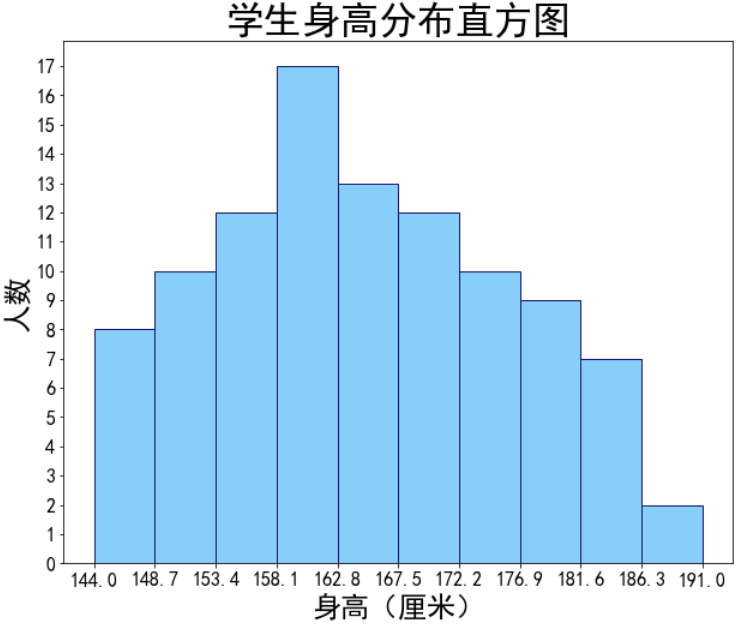
\includegraphics[width=0.64\textwidth]{直方图1.png}
\end{figure}

直方图比分位数表格更直观、更容易理解。我们可以直接看出,学生身高在$[158.1, \,\, 162.8)$区间最为集中,共有$17$人的身高落在这个区间里;
在$[186.3, \,\, 191]$区间最为稀疏,只有$2$人的身高落在这个区间里。

\begin{sk}
    \mbox{} \\
    \indent 1. 能否把分位数表格的信息用图表形式展示?\\
    \indent 2. 绘制直方图时,是否有别的方式划分区间?\\
    \indent 3. 分位数表格和直方图有什么联系?\\
    \indent 4. 直方图划分的区间个数是否越多越好?你认为应该如何确定划分的区间数?
\end{sk}

\begin{xt}
    \mbox{} \\
    \indent 1. 写出右分位数的自然定义。\\
    \indent 2. 写出顺右分位数的定义。
\end{xt}

\section{数据的结构}

\chapter{运动和优化}
\section{函数、图像和运动}
\section{极值原理}
\section{优化}

\chapter{数学和社会}
\section{随时代变化的数学}
\section{数学和科学}
\section{数学和现代化}

\end{document}